\chapter{INTRODUCTION}
\label{chap:intro}

The approach to big datasets has inspired new opportunities and challenges for Computer Science, Mathematics and Statistics People to reexamine how to apply convention of the fields to make big data technology beneficial to society. Atmosphere and oceanographic science disciplines are experiencing this information blast and are attempting to grow rapidly. Extraordinary measures of information are made accessible by administrative offices like \gls{nasa} and \gls{noaa}, and strongly utilized by mainstream researchers to make new development. The application of standard measures and procedures should be enhanced to deal with a flood of new information management. The methods used to envision and recover these information should be rethought. Worldwide expectations require current mobile application innovations for expert and novice to get information rapidly, precisely, and as effortlessly as possible as could be expected under the circumstances. \\
Conventional strategies for parsing through a remote/nearby document of records, choosing significant documents, opening the documents and performing examination on a solitary \gls{pc} don't scale with enormous information. Researchers are investing more energy exploring new information as opposed to working with the information already available. More disturbing still, beginners, specialists, and potential researchers get baffled and abandon utilizing these rich information. Toolboxes web applications and mobile applications are recommended in this proposal to alleviate this weight. Present day mobile application technology gives the network a dynamic stick to enable them to swim through the huge information soil. Figure~\ref{fig:gis_world} represents the connection of \gls{gis} with the world in different ways.

    \begin{figure}[H]
            \centering
            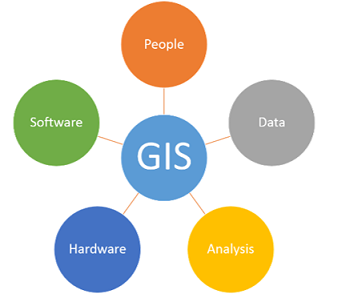
\includegraphics[width=0.50\linewidth]{figures/ch1/gis.png}
            \caption{\label{fig:gis_world} GIS connecting world in different ways \cite{CDC}}
    \end{figure}

\section{Background and significance of visualizing spatial data using smart phones}

According to the paper published in December 2014\cite{GSR_3}, The fields of Geo-information innovation and cartography have seen sensational changes in the last decade. In the past, \gls{gis} was an instrument only specialists used with the help of top of the line machines. In the mid nineties the work area of \gls{gis} appeared, which was anything but difficult to utilize and encourage with the Internet and Web mapping. \\
Despite late advances in touch pens as well as touch screens and the quick appropriation of these gadgets in ordinary life, we are a long way from utilizing the maximum capacity of cell phones in fulfilling the developing interest for visual access to information. With the Internet being accessible on cell phones, the industry is peering toward at the marriage of Geo-information administrations and cell phones as \gls{lbs}. "The rise of portable registering and remote gadgets has realized an entire palette of new potential outcomes and chances for Geo-information science and cartography". It has been expressed that in the coming time cartographic information isn't \gls{pc} driven however would be accessible on versatile frameworks situated at the purpose of estimation or use in the field. \\
Government organizations deliver basic information about the country's population, economy, administrations, agriculture and assets. These organizations are under pressure, both societal and money related in nature, to create and actualize \gls{ict}, inside and encompassing their organizations, supporting another worldview of society and modernization, focused on electronic open administration. In these last years, a surprising accomplishment in the utilization of hand-held portable PCs — cell phones, tablet \gls{pc}s, and \gls{pdi} has been seen for information gathering in various fields.
Information accumulation is perceived as a standout amongst the most tedious, costly and mistake given errands in any information stock venture. Hand-held PCs hold the potential to lessen the pressure of utilising the information for Government ogranizations, cost, and blunder rate of paper-based strategies for information accumulation. The great proceeding with development of the \gls{is} industry makes openings and difficulties for intriguing programming applications advancements and usage. In this sense, \gls{gis} and the electronic open organization administrations come into a circle. \gls{gis} information frameworks effectively store, control, join, and interrelate spatial genuine articles (e.g. political limits, streets, offices areas). Spatial information expressed with other information sources gives proficient intends to arranging, basic leadership, and administration numerous parts of financial exercises which take advantage of a spatial measurement.

Portable devices and equipment are changing the manner in which mapping innovation is being utilized by moving \gls{gis} from the work area into the client's hands, giving adaptability in information securing, information precision and uprightness — approval progressively lessening blunders and process costs — more data with significantly less time and exertion, quicker correspondence conventions, and high profitability, making the portability a tempting part of \gls{gis}.

\subsection{Past work}

Flashbackward to the appearance of the main Iphone in June 2007, the start of the cell phone insurgency. One year after, in July 2008, the Apple App Store was launched. It included 552 applications and 135 of them were free. After two months, the App Store's most prominent rival was launched, the Android Market. After the arrivals of these two technologies, the Windows application store came into market in October 2010 and was trailed by the Amazon application store in March 2011. The development and advancement of portable applications have not backed off. In May of that equivalent year, Gmail turns into the primary independent application to hit 1 billion downloads. \\
Talking more about mobile technologies, applications began as a stripped down, single-work program to keep running on the telephone. However, with advances in equipment and programming the pattern has moved back to having applications accomplish more tasks simultaneously. By including visual and spatial information in a portable application, they can build up a 3-D execution which can furnish the versatile application clients in a better way. The improvement of a versatile application for any data delivery gives a case of how to coordinate with the data which is stored on the servers with visual and spatial information to accomplish virtual experience.

Significant issues that portable innovation faces in its initial occasions are portrayed as underneath.

\begin{itemize}
  \item Geo-representation for little displays of cell phones was confined by few limitations, for example, the small screen size, absence of advance processor and memory, and the battery life.
  
  \item The ease of use of versatile Geo-perception arrangements was upset by insufficient ways to represent spatial data visually. The causes were either the utilization of checked paper maps intended for a medium with various attributes or the creation of obscured and jumbled maps that fit an extensive screen, however not the little cell phone screen with lower processors.
  
  \item The bad network speed with surprising expense of smart phones were one of the real issues that were looked by individuals creating applications.
\end{itemize}

\subsection{Current scenario}

Despite late advances in mobile application field, we are a long way from utilizing the maximum capacity of cell phones in fulfilling the developing interest for visual access to information. Ongoing advancements in technology have demonstrated that systems of making and utilizing maps have changed fundamentally. The fields of getting, overseeing, investigating, intuitiveness and envisioning a lot of Geo-spatial information have seen exceptionally energetic and critical improvement throughout the most recent two decades and it's quickly evolving. The ubiquity of hand held gadgets and portable Internet gives another stage to Geo-information. The cartographic presentation and plan for these little gadgets is a test because of their impediments.

Prior to the development of cell phones, information representation's source was the \gls{pc}, for which the most part was conveyed through programs and client-server applications. Be that as it may, when seen on smart gadgets, information perceptions in PC-particular applications are hard to peruse, explore and utilize. A bit of the present flexible applications in the market for data visualization are:

\begin{itemize}
  \item "\gls{gis} Cloud Mobile Data Collection" is a tool for today’s mobile devices which enables you to collect data and conduct field surveys faster and easier than ever before. Combined with powerful new custom mobile and web forms, the new Mobile Data Collection app can also be highly tailored for your mobile workforce and a wide variety of applications in minutes without any programming. \cite{GIS_cloud_mobile_data_collection}
 
  
  \begin{figure}[!htb]
        \begin{minipage}{0.35\textwidth}
            \centering
            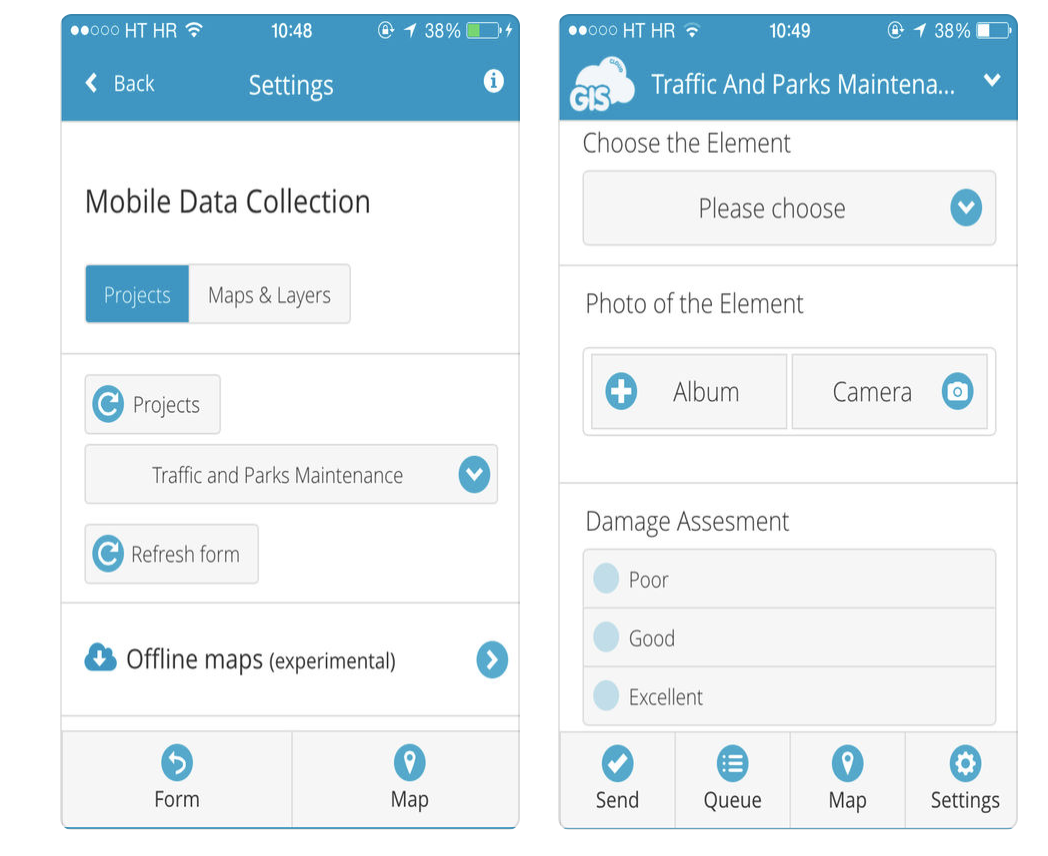
\includegraphics[width=1.0\linewidth]{figures/ch1/mobile_data_collection_1.png}
            \caption{Mobile data collection application screenshot - 1 \cite{GIS_cloud_mobile_data_collection}}\label{Fig:mobile_data_collection_1}
        \end{minipage}\hfill
        \begin{minipage}{0.35\textwidth}
            \centering
            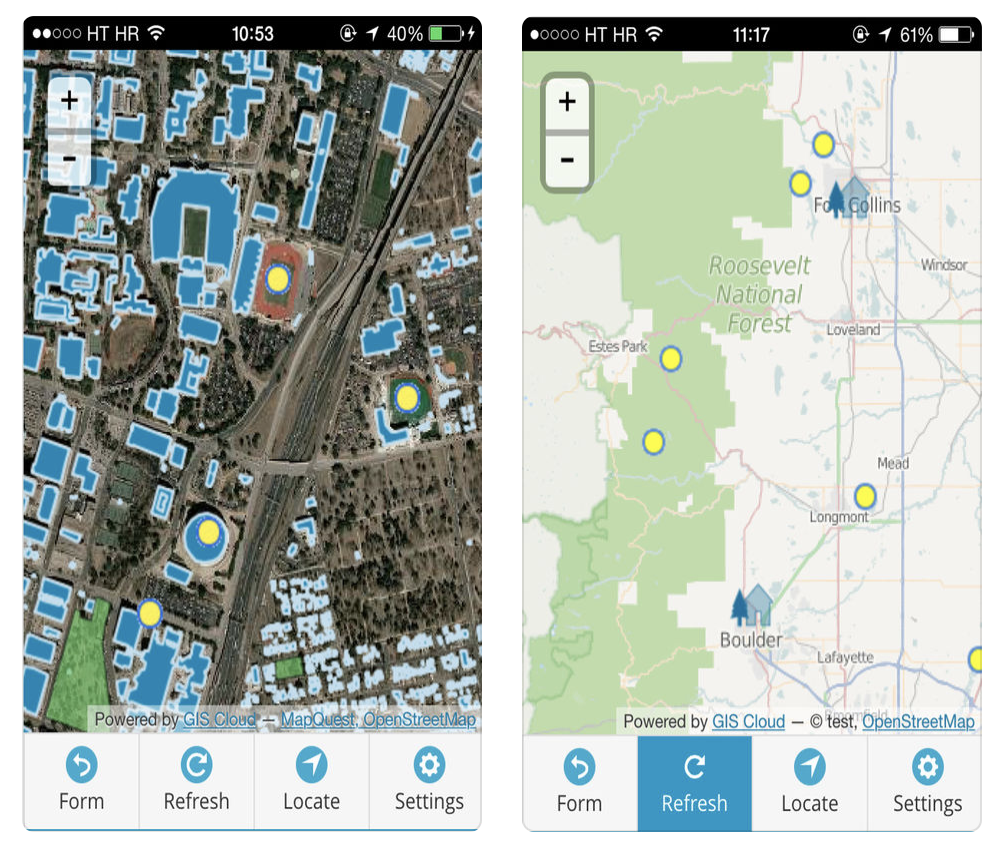
\includegraphics[width=1.0\linewidth]{figures/ch1/mobile_data_collection_2.png}
            \caption{Mobile data collection application screenshot - 2 \cite{GIS_cloud_mobile_data_collection}}\label{Fig:mobile_data_collection_2}
        \end{minipage}
\end{figure}

  
  \item The "Spatial Agent" Mobile App has been created to exploit new capacities to picture this developing scope of spatial and transient advancement related information on versatile stages. This App shows a basic yet greatly ground-breaking way to deal with imagine a scope of open area spatial data sets through intuitive maps and graphs to take into account information representation at various scales and ranges. The methodology actually puts the globe in the clients hands and enables one to get to an expanding gathering of open space multisectoral data sets (counting at worldwide, provincial, and national levels) being produced for use of different improvement related foundations and governments over the world. So whether the user is keen on water assets or environmental change, catastrophe administration or general advancement, this is an unquestionable requirement having application. The straightforwardness of utilization and abundance of data is certain to interest anyone regardless of the level of expertise. Figure~\ref{fig:spatial_agent} shows the screenshot of the application. \cite{Spatial_Agent}

  \begin{figure}[H]
            \centering
            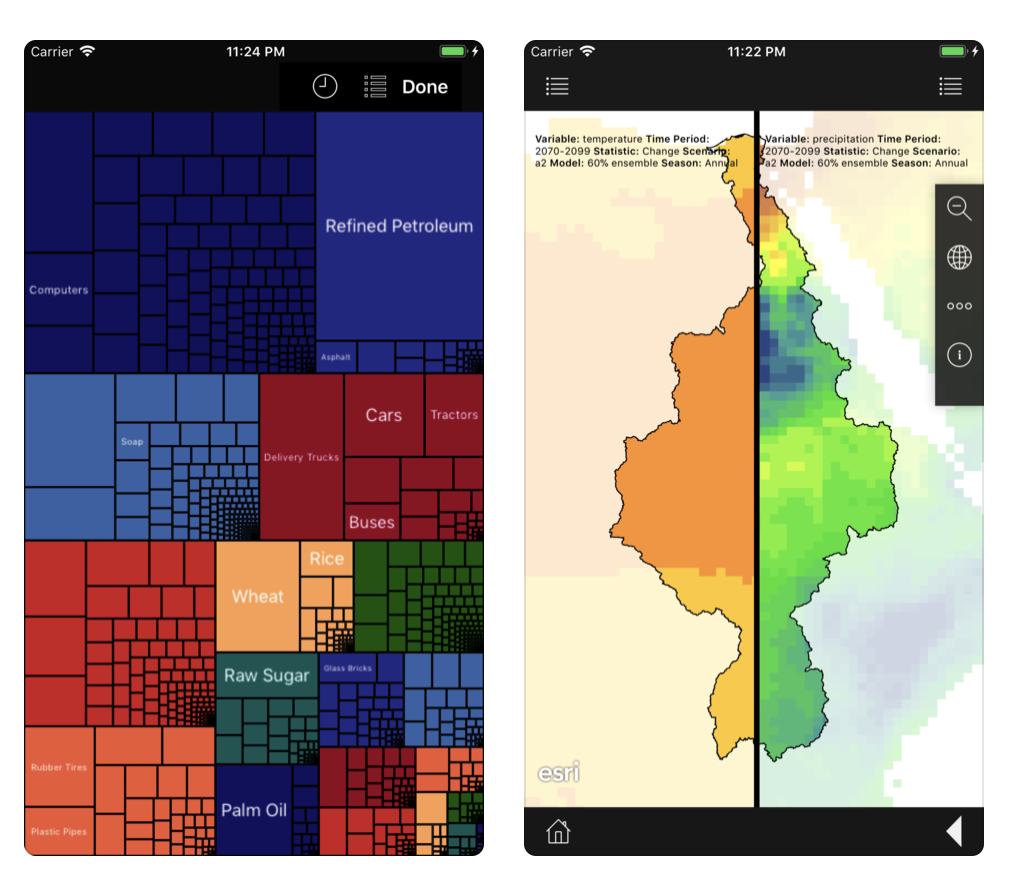
\includegraphics[width=0.5\linewidth]{figures/ch1/spatial_agent.png}
            \caption{\label{fig:spatial_agent} Spatial agent application screenshot \cite{Spatial_Agent}}
    \end{figure}
  
  \item \gls{gps} Another way of visualisation is by tracking for bike, hike, ski and outdoor activities. It is ideal for displaying a totally new perspective of the world on your iPhone screen.
  
    \begin{figure}[H]
            \centering
            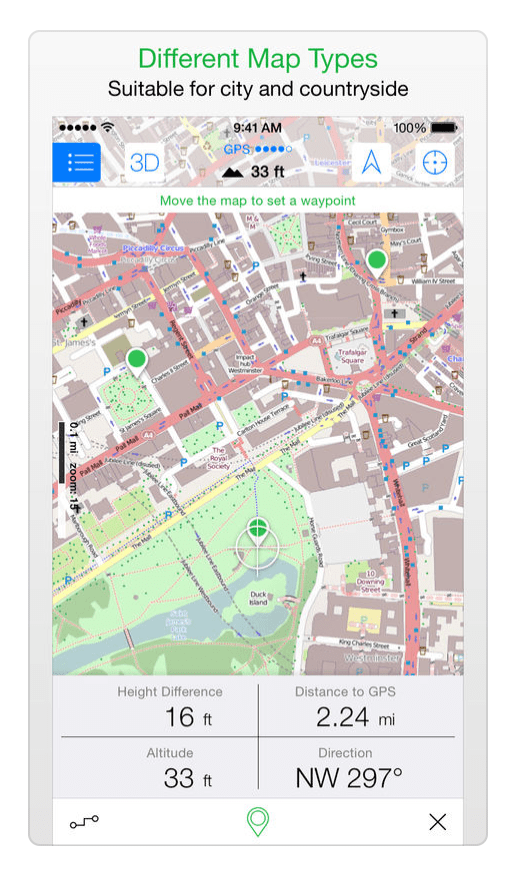
\includegraphics[width=0.25\linewidth]{figures/ch1/map_3d.png}
            \caption{\label{fig:map_3d} Maps 3D application screenshot \cite{Spatial_Agent}}
    \end{figure}
\end{itemize}

%figure of the app screens hots - search Maps 3D - Outdoor GPS app on app store and get screen shots
  
\subsection{Future work for quick visualization and analysis of big data}

There were 4.77 billion versatile application clients in 2017, and it is anticipated there will be 5.07 billion portable application clients in 2019 (eMarketer). Of these billions of clients, 66 percent of clients apportion the vast majority of their opportunity between gaming, stimulation, news, and sports applications (Think with Google). In a report by App Annie\cite{AppAnnie}, a normal US client spends more than 2.25 hours on applications and uses somewhere around 9 applications or more. As indicated by comScore's 2017 US Mobile App report, the 10 applications that command the United States space are: Facebook, Youtube, Facebook Messenger, Google Search, Google Maps, Instagram, Snapchat, Google Play, Gmail, and Pandora. \cite{eBiz_solutions}. \\
Of all the portable applications, a standout amongst the most valuable perspectives might be the power it needs to develop your business. Applications enable you to traverse your day by day exercises, similar to messages, exercises, and mingling. So why not let it enable you to extend your business? One of the prominent misinterpretations is that applications are intended for huge brand organizations. In spite of the fact that, that isn't the situation. The greatest favorable position of having a versatile application is the immediate association with the clients. It enables you to showcase new highlights, items, arrangements, or reliability programs truly into the palm of your gathering of people's hands.

\textbf{The Technology Trends:} The \gls{ngac} has pinpointed five innovation inclines that are encouraging, organizing, and driving improvement in geospatial advancements which are mentioned below. 

\begin{itemize}
  \item \textbf{The Real-Time Revolution} \\
 Real time spatial information is currently being produced universally and its applications in research and business are quickly approaching across the board. The capacity to cooperate continuously with this information is an ongoing marvel. This development is working as a center change specialist in geology, cartography, GIScience, and many related geospatial fields. It is significantly realigning conventional connections and structures; growing examination skylines; and changing the manners by which geographic information is presently gathered, mapped, demonstrated, and utilized in geology and science and society all the more comprehensively. This prompt collaboration among space and time remains the hidden procedure that is creating the ebb of combined spatiotemporal information, new geographic research activities, and heap versatile geospatial applications in governments, organizations, and society. 
  
  \item  \textbf{Scaling down of Technologies} \\
 The ability to make little and frequently cheap gadgets and sensors with remote availability is driving a blast of the \gls{IoT}.
  
  \item  \textbf{Multiplication of New Mobile Geo spatial Sensor Platforms} \\
  The reduction in spatial data sensor platforms innovations has made it practical to investigate new modalities for sensor dissemination, for example, little satellites (smallsats) and unmanned flying machine frameworks (UAS, or automatons) that can be quickly composed and sent with circles or flight ways custom fitted to the mission. These portable geospatial sensor stages extraordinarily extend the capacities of people, organizations, and governments to gather volumes of remotely detected information for various and mission-basic purposes, including catastrophe reaction, ecological checking, and open security. 
  
  \item  \textbf{Extending Wireless and Web Networks} \\
 Quicker and more extensive remote and web systems are starting to address to a limited extent, the developing interest for enhanced techniques for information transmission and geospatial information conveyance to end clients. This is laying the basis for governments and shoppers around the globe to more comprehensively offer by utilizing spatiotemporal information, including for constant applications. 
  
  \item  \textbf{Advances in Computing Capacity for Geospatial Research, Apps} \\
 Superior registering systems (counting CyberGIS) and distributed computing administrations (counting cloud GIS) are giving governments and others conductors through which they can all the more effortlessly and rapidly access and add to developing vaults of Geo-spatial information, instruments, and administrations.
  
\end{itemize}

\section{Motivation of the VACYD research: crop yield data visualization}

The purpose of this research is to make crop data reach as many people as possible by providing an easy user-friendly, fast, reliable visualization. The paper's author's interest in \gls{iOS} drove this project to be developed in native \gls{iOS} platform. App Solutions, a software company has explained the advantages / disadvantages of making native \gls{iOS} application over Android also shown in Figure 1.7\cite{theAPPsolutions}.

  \begin{figure}[H]
            \centering
            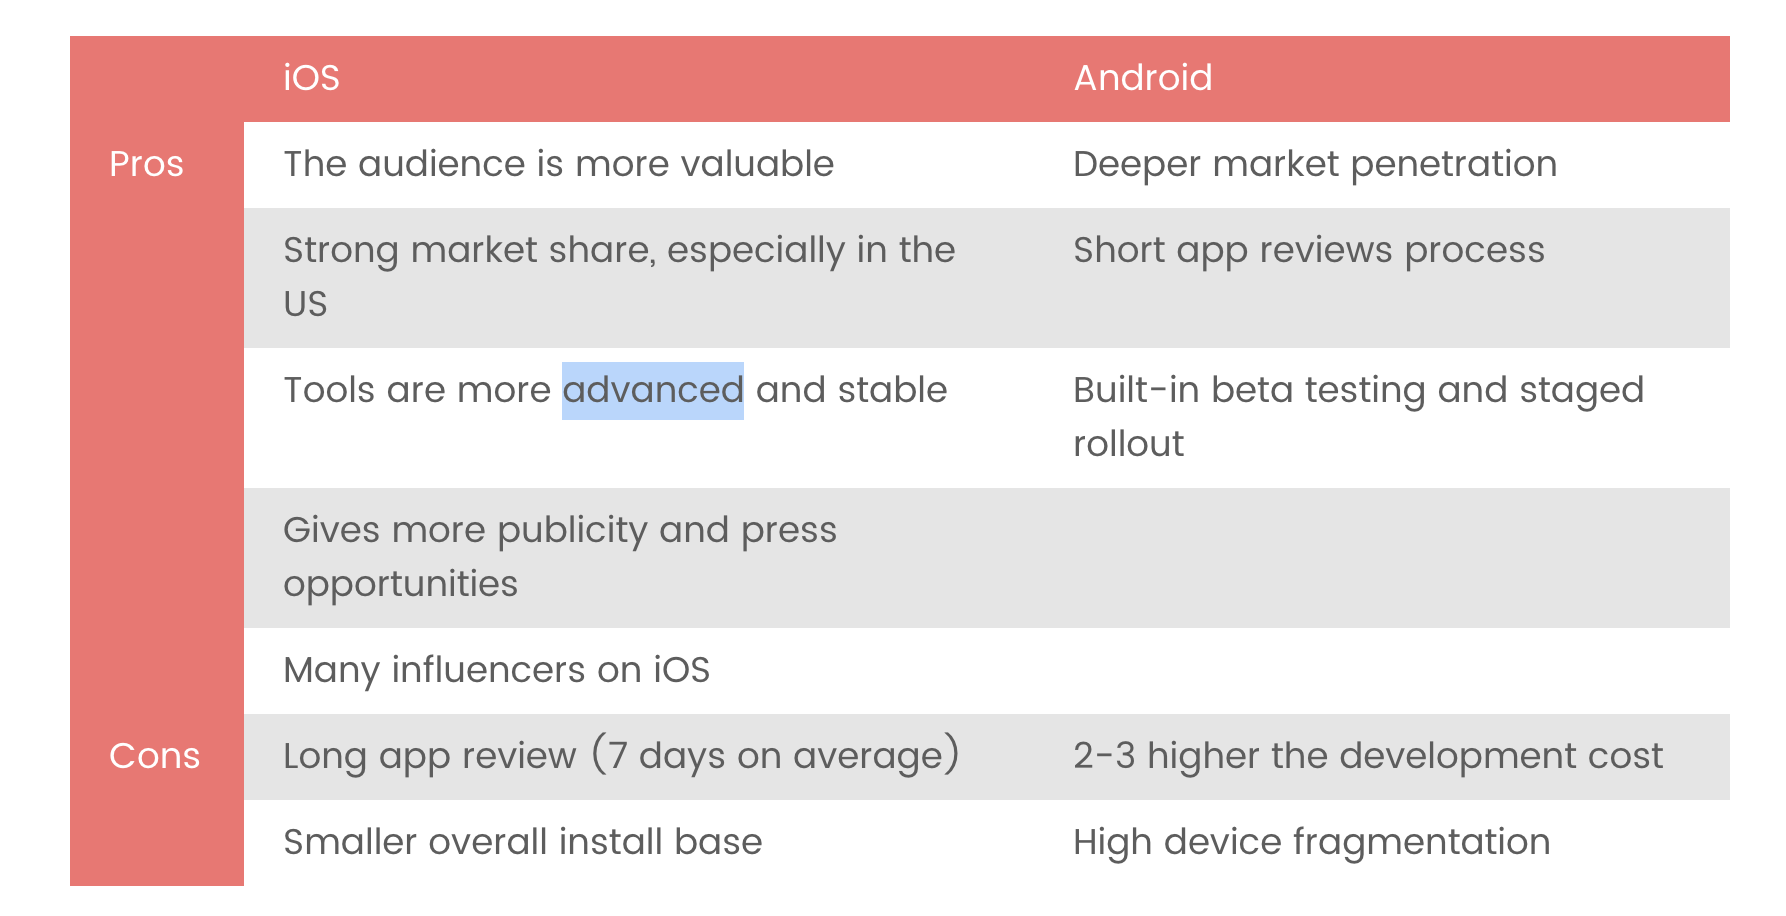
\includegraphics[width=0.8\linewidth]{figures/ch1/iosVSandroid.png}
            \caption{\label{fig:iosVSandroid} Advantages/Disadvantages of developing native iOS \& Android application \cite{theAPPsolutions}}
  \end{figure}


\section{A short summary of the app development method and results}

Every day many great versatile applications are distributed to the Google Play and Apple App Stores. A portion of these versatile applications are diversions, others are interpersonal organizations, and many are web based business applications. These applications, if professionally fabricated, ought to pursue a comparative portable application advancement process. This versatile application advancement process regularly incorporates thought, methodology, plan, improvement, arrangement, and post-dispatch stages.

There are various methodologies, advancements, and programming dialects that can be utilized to fabricate a versatile application. Some may be less expensive to utilize, yet are less performant, though others may take more time to execute and be pointless excess. The most noticeably bad plausibility is expanding on a withering or untrustworthy innovation stack. In the event that you commit this error, you may need to remake your application or pay a premium for designers pushing ahead.

For front-end improvement, there are essentially three approaches. They are stage particular local, cross-stage local, and crossover. Here is a concise outline of each methodology and a few articles that dig into each with more noteworthy subtle elements.

%data visual why people like hybrid native
\begin{itemize}
  \item \textbf{Platform-specific Native} \\
  Apps worked with this methodology are composed independently for every versatile stage. Code can't be reused among Android and iOS, yet these applications can be individually very similar. The \gls{ui} can look altogether local (so it will fit in with the OS) and the application should work smoothly. This is frequently the most costly methodology, yet is extremely attempted and tried.
  
  \item \textbf{Cross-platform Native} \\ 
  Apps worked with this methodology have a few (or altogether shared) code, yet run locally in their own operating systems. Regular advancements utilized for this are React Native, Xamarin, and Native Script. This is a decent center ground between the different methodologies in that it is more financially savvy, however can even now be upgraded and styled for every stage.
  
  \item \textbf{Hybrid} \\
 Cross breed applications are manufactured utilizing web innovations such as \gls{html}, \gls{css}, Javascript and are introduced by means of a local wrapper. This should be possible utilizing advancements, for example, Cordova, Phone Gap, and Ionic. Although this choice is the least expensive, it shows troubles.
\end{itemize}

We have picked native application for the venture just due to following reasons.

\begin{itemize}
  \item \textbf{Native features} \\ 
  There are numerous local highlights i.e. Camera, Document Directory access, Hardware Device Buttons, \gls{gpu} usage and so forth which you could conceivably approach on the chance that you get your application created utilizing Hybrid innovation, contingent upon the structure that you embrace to create.
  
  \item \textbf{User experience} \\ 
  In the event that you are building up an application that requires some imaginative client encounter, don't think much and go for local application advancement. Cross breed application can never coordinate the level of imaginative client encounter that you get in local applications.
  
  \item \textbf{Speed and Performance} \\
 With advancement in the field of mobile applications, everything is viewed as including the memory and battery of the cell phone. In addition to the fact that it is less demanding to execute motions, the code works quicker, new capacities will incorporate faster, and the following topographical area likewise stays basic.
 
\end{itemize}
